\chapter{Ingeniería genética y biotecnología}\label{ch:b3:genetic-engineering}

Hasta 1982 todos los diabéticos del mundo seguían vivos gracias a
insulina extraída del páncreas de cerdos y de vacas --- unos ocho mil
kilogramos de glándulas por cada kilogramo de hormona --- y una parte de
los pacientes reaccionaba contra la proteína ajena. Ese año llegó al
mercado el primer fármaco fabricado por un organismo modificado
genéticamente: la insulina humana, sintetizada por \emph{Escherichia
coli} con el gen humano en un \omterm{def:b3:genetic-engineering:tools}{plásmido}. Las herramientas que lo hicieron
posible se habían reunido a lo largo de la década anterior --- enzimas
que cortan el ADN en secuencias elegidas, enzimas que unen los trozos,
\omterm{def:b3:genetic-engineering:tools}{plásmidos} que los llevan a una célula y los copian allí --- y se les
sumaron en las siguientes la \omterm{def:b3:genetic-engineering:pcr}{reacción en cadena de la polimerasa}, la
inyección de genes en embriones y, desde 2012, un sistema inmunitario
bacteriano convertido en unas tijeras programables capaces de reescribir
una letra de un genoma en una célula viva. Este capítulo trata de esas
herramientas, de la aritmética que gobierna su uso y de lo que se ha
construido con ellas, desde un ratón luminoso hasta una cura para la
anemia falciforme.

\section{Cortar, unir y copiar ADN}

\begin{definition}[Enzimas de restricción, ligasa y vectores]\label{def:b3:genetic-engineering:tools}
\index{enzima de restricción}\index{extremo cohesivo}\index{ADN-ligasa}\index{vector}\index{plásmido}\index{marcador de selección}
Una \emph{enzima de restricción} de tipo~II es una endonucleasa
bacteriana que corta el ADN de doble hebra en una secuencia concreta de
\numrange{4}{8} pares de bases, casi siempre un palíndromo: EcoRI corta
G$^{\downarrow}$AATTC y deja salientes de hebra sencilla de cuatro bases
(\emph{extremos cohesivos}) complementarios de cualquier otro extremo
EcoRI; otras enzimas dejan \emph{extremos romos}. La \emph{ADN-ligasa}
sella dos fragmentos cuyos extremos encajan. Un \emph{vector} es una
molécula de ADN que se replica en un hospedador y puede llevar un
fragmento insertado: un \emph{plásmido} de unas pocas kilobases con un
origen de replicación, un \emph{marcador de selección} (un gen de
resistencia a un antibiótico, de modo que solo crecen en el antibiótico
las células que tomaron el plásmido) y un grupo de sitios de restricción
únicos para el inserto; el bacteriófago $\lambda$, los cósmidos y los
cromosomas artificiales bacterianos o de levadura para insertos de
\qtyrange{20}{1000}{kb}. El ADN entra en una bacteria por
\emph{transformación}, tras un choque químico o eléctrico que hace la
membrana transitoriamente permeable, con una eficiencia de $10^{6}$ a
$10^{9}$ transformantes por microgramo de plásmido. Una molécula
\emph{recombinante} es la que une ADN de dos procedencias.
\end{definition}

\begin{proof}[Evidencia]
Cohen, Chang, Boyer y Helling (1973) cortaron con EcoRI el \omterm{def:b3:genetic-engineering:tools}{plásmido}
pSC101 y un segundo \omterm{def:b3:genetic-engineering:tools}{plásmido} con otro gen de resistencia, mezclaron y
ligaron los fragmentos, transformaron \emph{E.~coli} y recuperaron
colonias resistentes a ambos antibióticos que llevaban un solo \omterm{def:b3:genetic-engineering:tools}{plásmido}
hecho de los dos --- el primer ADN recombinante que se replicó en una
célula. Al año siguiente insertaron en pSC101 genes de ARN ribosómico de
un sapo y mostraron que el ADN del anfibio se replicaba, y se
transcribía, en la bacteria: los genes cruzan sin cambios la frontera
entre reinos, y una bacteria copiará el ADN que se le dé.
\end{proof}

\begin{omfigure}
\begin{tikzpicture}[every node/.style={font=\scriptsize}, >=stealth]
  % plasmid circle
  \draw[very thick, omDef] (0,0) circle (1.8);
  % ori
  \draw[very thick, omMeth!70!black] (0,0) ++(60:1.8) arc[start angle=60, end angle=100, radius=1.8]; \node[above right] at (80:1.95) {origen de replicación};
  % ampR
  \draw[very thick, omProp] (0,0) ++(160:1.8) arc[start angle=160, end angle=250, radius=1.8]; \node[left, align=right] at (205:2.0) {gen de\\resistencia (marcador)};
  % MCS with insert
  \draw[very thick, omThm] (0,0) ++(-40:1.8) arc[start angle=-40, end angle=10, radius=1.8]; \node[right, align=left] at (-15:2.0) {inserto, ligado en\\el sitio de restricción};
  \draw[omThm] (-40:1.7) -- (-40:1.95); \draw[omThm] (10:1.7) -- (10:1.95);
  \node at (0,0.25) {plásmido}; \node at (0,-0.15) {\qtyrange{3}{5}{kb}};
  % sticky ends detail
  \begin{scope}[xshift=5.7cm, yshift=0.8cm]
    \node[left, align=right] at (-0.2,0) {EcoRI};
    \node[font=\ttfamily\scriptsize, anchor=west] at (0,0.25) {5$'$-G\,\textcolor{omThm}{AATT}C-3$'$};
    \node[font=\ttfamily\scriptsize, anchor=west] at (0,-0.25) {3$'$-C\textcolor{omThm}{TTAA}\,G-5$'$};
    \draw[->, omThm, thick] (0.62,0.55) -- (0.62,0.3); \draw[->, omThm, thick] (1.62,-0.55) -- (1.62,-0.3);
    \node[anchor=west, align=left] at (2.6,0) {corte escalonado:\\salientes de 4 bases\\complementarios:\\extremos cohesivos};
  \end{scope}
  \begin{scope}[xshift=5.7cm, yshift=-1.3cm]
    \draw[very thick, omDef] (0,0.15) -- (1.2,0.15); \draw[very thick, omDef] (0,-0.15) -- (0.7,-0.15);
    \draw[very thick, omThm] (1.7,0.15) -- (3.0,0.15); \draw[very thick, omThm] (1.2,-0.15) -- (3.0,-0.15);
    \node[above] at (1.45,0.2) {hibridan}; \node[below, align=center] at (1.5,-0.25) {dos extremos EcoRI cualesquiera se aparean;\\la ligasa sella el esqueleto};
  \end{scope}
\end{tikzpicture}

{\small Un \omterm{def:b3:genetic-engineering:tools}{vector} de clonación y su química. El \omterm{def:b3:genetic-engineering:tools}{plásmido} lleva un origen,
un \omterm{def:b3:genetic-engineering:tools}{marcador de selección} y un sitio de restricción único en el que se
liga un fragmento cortado con la misma enzima; los \omterm{def:b3:genetic-engineering:tools}{extremos cohesivos}
hacen compatibles dos fragmentos cualesquiera cortados por la misma
enzima.}
\end{omfigure}

\begin{method}[Clonar un gen]\label{met:b3:genetic-engineering:cloning}
\index{clonación}\index{genoteca}\index{cribado}
(1) Obténgase el inserto: córtese ADN genómico con una \omterm{def:b3:genetic-engineering:tools}{enzima de
restricción}, o cópiese el ARN mensajero en ADN complementario (ADNc, que
carece de intrones y por tanto puede expresarse en bacterias), o
amplifíquese el gen por PCR con \omterm{def:b3:genetic-engineering:pcr}{cebadores} que lleven sitios de
restricción. (2) Córtense el \omterm{def:b3:genetic-engineering:tools}{vector} y el inserto con la misma enzima o
enzimas --- dos enzimas distintas fuerzan la orientación del inserto ---
y líguense. (3) Transfórmense bacterias y siémbrense en el antibiótico:
solo crecen las células con \omterm{def:b3:genetic-engineering:tools}{plásmido}. (4) Distínganse los \omterm{def:b3:genetic-engineering:tools}{plásmidos} con
inserto de los que se cerraron sobre sí mismos: con un gen marcador
interrumpido por el sitio de clonación (\emph{lacZ}: las colonias blancas
tienen inserto y las azules no). (5) Críbense las colonias buscando el
inserto deseado: por hibridación con una sonda marcada, por PCR o por
digestión con \omterm{def:b3:genetic-engineering:tools}{enzimas de restricción} y electroforesis en gel.
(6) Secúnciese el inserto. Una \emph{genoteca} es el conjunto de clones
de todo un genoma o transcriptoma, del que puede pescarse cualquier gen
con el mismo cribado.
\end{method}

\begin{omfigure}
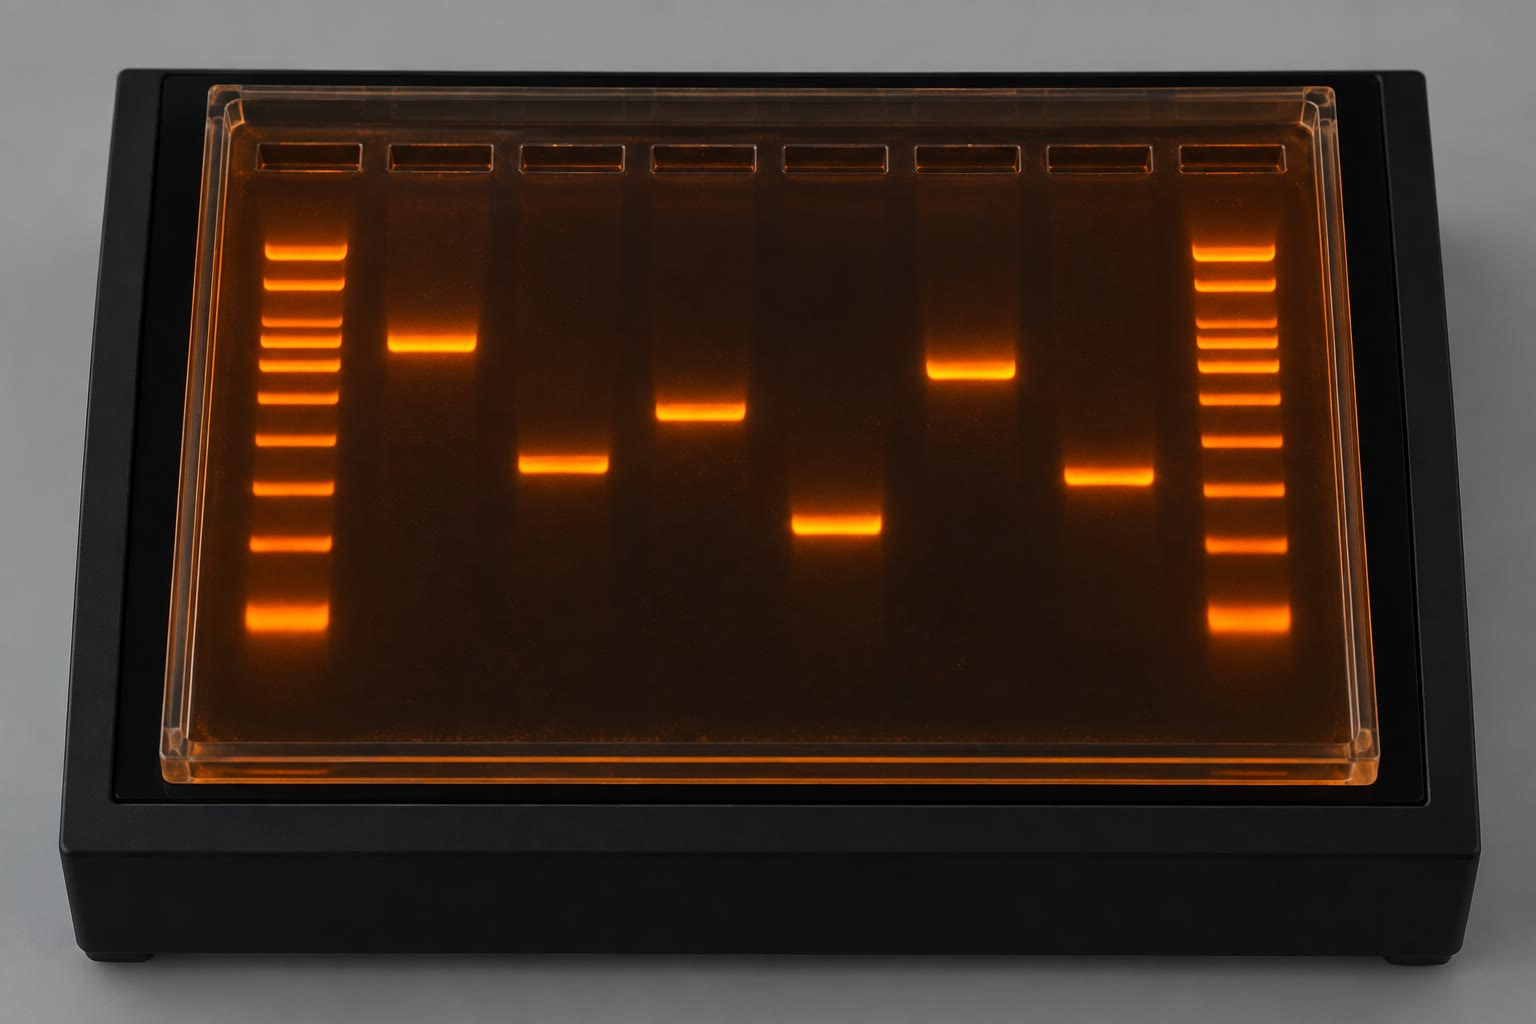
\includegraphics[width=0.56\linewidth]{images/book5/ai/b5-06-agarose-gel.jpg}

{\small Un gel de agarosa bajo luz ultravioleta: los fragmentos de ADN
migran hacia el ánodo a una velocidad que cae con su longitud, de modo
que cada banda es una población de moléculas de un solo tamaño, comparada
con la escalera de tamaños conocidos de las calles exteriores.}
\end{omfigure}

\begin{definition}[La reacción en cadena de la polimerasa]\label{def:b3:genetic-engineering:pcr}
\index{reacción en cadena de la polimerasa}\index{cebador}\index{PCR cuantitativa}
La \emph{reacción en cadena de la polimerasa} (PCR) amplifica un tramo
elegido de ADN situado entre dos \emph{cebadores} --- oligonucleótidos
sintéticos de unas veinte bases complementarios de las dos hebras en los
extremos de la diana --- mediante ciclos de tres temperaturas:
\qty{95}{\celsius} para separar las hebras,
\qtyrange{50}{65}{\celsius} para que los cebadores hibriden y
\qty{72}{\celsius} para que una polimerasa termoestable (la Taq, de la
bacteria de aguas termales \emph{Thermus aquaticus}) los alargue. Cada
ciclo duplica el número de copias del segmento situado entre los
cebadores, de modo que treinta ciclos convierten una sola molécula en mil
millones. La \emph{PCR con transcripción inversa} copia primero el ARN en
ADN y mide así transcritos o virus de ARN; la \emph{PCR cuantitativa}
(qPCR) sigue la amplificación en tiempo real con un colorante fluorescente
y lee la cantidad inicial a partir del ciclo en que la señal cruza un
umbral.
\end{definition}

\begin{theorem}[La aritmética de la amplificación]\label{thm:b3:genetic-engineering:pcr}
\index{ciclo umbral}
Con una eficiencia $E$ por ciclo ($E = 1$ para una duplicación perfecta),
$N_{0}$ copias iniciales pasan a ser
\[
N_{n} = N_{0}\,(1 + E)^{n}
\]
tras $n$ ciclos. Si la fluorescencia cruza un umbral fijo cuando el
número de copias llega a $N_{T}$, el \emph{\omterm{thm:b3:genetic-engineering:pcr}{ciclo umbral}} es
\[
C_{T} = \frac{\log N_{T} - \log N_{0}}{\log(1 + E)},
\]
una recta en $\log N_{0}$ de pendiente $-1/\log(1+E)$: para $E = 1$, cada
aumento de diez veces de la cantidad inicial baja $C_{T}$ en
$\log_{2} 10 = 3.32$ ciclos, y dos muestras cuyos \omterm{thm:b3:genetic-engineering:pcr}{ciclos umbral} difieren
en $\Delta C_{T}$ difieren en copias iniciales por el factor
$(1 + E)^{\Delta C_{T}}$.
\end{theorem}
\begin{proof}
Cada ciclo multiplica el número de copias por $1 + E$, de modo que
$N_{n}$ es una sucesión geométrica. Igualando $N_{n} = N_{T}$ y
despejando $n$ se obtiene $C_{T}$; la pendiente es el coeficiente de
$\log N_{0}$. Para dos muestras,
$C_{T,1} - C_{T,2} = (\log N_{0,2} - \log N_{0,1})/\log(1+E)$, de donde
$N_{0,2}/N_{0,1} = (1+E)^{\Delta C_{T}}$.
\end{proof}

\begin{example}[Leer una placa de qPCR]\label{ex:b3:genetic-engineering:qpcr}
Una prueba de ARN vírico cruza el umbral en el ciclo $22$ en un paciente
y en el $32$ en otro; con $E \approx 1$ el primero lleva $2^{10}
\approx 1000$ veces más virus. Una muestra de diez copias cruza hacia el
ciclo $37$ cuando el umbral está en $10^{12}$ copias ($\log_{2} 10^{11} =
36.5$); una carrera de $40$ ciclos detecta por tanto unas pocas
moléculas, y también lo hace una sola molécula contaminante de un
amplicón anterior, que es por lo que los laboratorios separan las salas
donde se monta la PCR de aquellas donde se manipulan los productos.
\end{example}

\begin{omfigure}
\begin{tikzpicture}
\begin{axis}[
  width=0.7\linewidth, height=5.6cm,
  axis x line=bottom, axis y line=left,
  xmin=0, xmax=40, ymin=1, ymax=1e14, ymode=log,
  xlabel={ciclo}, ylabel={copias},
  xlabel style={font=\small, at={(axis description cs:0.5,-0.12)}, anchor=north},
  ylabel style={font=\small},
  tick label style={font=\small}, xtick={0,10,20,30,40},
  clip=false,
]
\addplot[very thick, omDef, domain=0:40, samples=41] {1e7*2^x/(1+2^x/1e5)};
\addplot[very thick, omThm, domain=0:40, samples=41] {1e4*2^x/(1+2^x/1e8)};
\addplot[very thick, omMeth!70!black, domain=0:40, samples=41] {10*2^x/(1+2^x/1e11)};
\addplot[dashed, gray, domain=0:40, samples=2] {1e12};
\node[font=\scriptsize, gray, anchor=south west] at (axis cs:0.5,1.3e12) {umbral $N_{T}$};
\draw[gray] (axis cs:16.6,1) -- (axis cs:16.6,1e12); \draw[gray] (axis cs:26.6,1) -- (axis cs:26.6,1e12); \draw[gray] (axis cs:36.5,1) -- (axis cs:36.5,1e12);
\node[font=\scriptsize, anchor=south] at (axis cs:16.6,3e12) {$C_{T} = 16.6$}; \node[font=\scriptsize, anchor=south] at (axis cs:26.6,3e12) {$26.6$}; \node[font=\scriptsize, anchor=south] at (axis cs:36.5,3e12) {$36.5$};
\end{axis}
\end{tikzpicture}

{\small Curvas de amplificación para $N_{0} = 10^{7}$ (azul), $10^{4}$
(rojo) y $10$ copias (verde), con $E = 1$ y la meseta que imponen los
reactivos. Una diferencia de mil veces en $N_{0}$ desplaza el \omterm{thm:b3:genetic-engineering:pcr}{ciclo
umbral} en $10$; las mesetas son todas iguales, y por eso el producto
final no dice nada sobre el punto de partida.}
\end{omfigure}

\section{Fabricar proteínas}

\begin{definition}[Sistemas de expresión]\label{def:b3:genetic-engineering:expression}
\index{vector de expresión}\index{proteína recombinante}\index{anticuerpo monoclonal}
Un \emph{\omterm{def:b3:genetic-engineering:tools}{vector} de expresión} sitúa la secuencia codificante clonada bajo
un promotor fuerte y controlable del hospedador (el promotor \emph{lac} o
el T7 en \emph{E.~coli}, inducidos por un análogo de azúcar), con un
sitio de unión al ribosoma, un terminador y a menudo una \emph{etiqueta}
--- seis histidinas, una proteína pequeña --- fusionada al producto para
purificarlo en una columna. Las bacterias fabrican gramos por litro de
una proteína sencilla (insulina, hormona del crecimiento, enzimas) pero
no pueden glicosilar ni plegar proteínas complejas de mamífero; la
levadura añade azúcares a su manera; y las células de insecto y de
mamífero (las de ovario de hámster chino son el estándar de la industria)
fabrican anticuerpos y factores de coagulación plegados y glicosilados
como en el ser humano. Un \emph{anticuerpo monoclonal} lo fabrica un
\emph{hibridoma} --- un linfocito~B productor de anticuerpos fusionado
con una célula de mieloma inmortal (Köhler y Milstein, 1975) --- o, hoy,
clonando los genes del anticuerpo en una línea de expresión de mamífero,
donde el armazón de ratón puede sustituirse por secuencia humana para
evitar el rechazo inmunitario (\cref{ch:b3:adaptive-immunity}).
\end{definition}

\begin{example}[La insulina]\label{ex:b3:genetic-engineering:insulin}
La insulina humana consta de dos cadenas, la A (21 residuos) y la B
(30), unidas por puentes disulfuro y cortadas en la célula $\beta$ a
partir de un único precursor, la proinsulina. El primer proceso expresó
las dos cadenas por separado en \emph{E.~coli}, cada una fusionada a la
$\beta$-galactosidasa, las separó químicamente y las unió in vitro; los
procesos posteriores expresan proinsulina y la cortan con las enzimas que
usa el páncreas. Desde 1996 se ha alterado la propia secuencia: cambiar o
añadir un residuo o dos da análogos que se disocian más deprisa (para una
comida) o que precipitan en el punto de inyección y se liberan a lo largo
de un día. Una proteína que costaba ocho toneladas de glándulas por
kilogramo se fabrica hoy en un fermentador, idéntica a la humana o mejor
que ella.
\end{example}

\section{Organismos transgénicos}

\begin{definition}[Transgénesis y direccionamiento génico]\label{def:b3:genetic-engineering:transgenic}
\index{organismo transgénico}\index{microinyección}\index{supresión génica}\index{célula madre embrionaria}\index{direccionamiento génico}
Un organismo \emph{transgénico} lleva un gen introducido en su línea
germinal, de modo que todas sus células lo tienen y se hereda. En los
ratones la vía clásica es la \emph{microinyección} del ADN en uno de los
pronúcleos de un huevo fecundado (Gordon y Ruddle, 1980), que se integra
en un sitio al azar en una fracción de los embriones; Palmiter y Brinster
(1982) hicieron ratones del doble del tamaño normal inyectando el gen de
la hormona del crecimiento de rata detrás de un promotor de
metalotioneína. El \emph{direccionamiento génico} sustituye o interrumpe
en cambio un gen elegido: se introduce en \emph{células madre
embrionarias} una construcción con brazos largos homólogos de la diana,
se seleccionan las raras células en las que la \omterm{def:b3:dna-repair:dsb}{recombinación homóloga} la
ha colocado en el lugar correcto y se inyectan en un blastocisto, y el
ratón quimérico resultante transmite el gen alterado (Capecchi, Smithies
y Evans, en los años ochenta). Una \emph{supresión génica} carece del
gen; una \emph{inserción dirigida} lleva una versión modificada; y un
alelo \emph{condicional}, flanqueado por sitios loxP, solo se suprime
donde y cuando se expresa la Cre (\cref{ch:b3:dna-repair}). Se han
suprimido unos diez mil genes de ratón, y para la mayoría el fenotipo fue
la primera indicación de lo que hace el gen.
\end{definition}

\begin{omfigure}
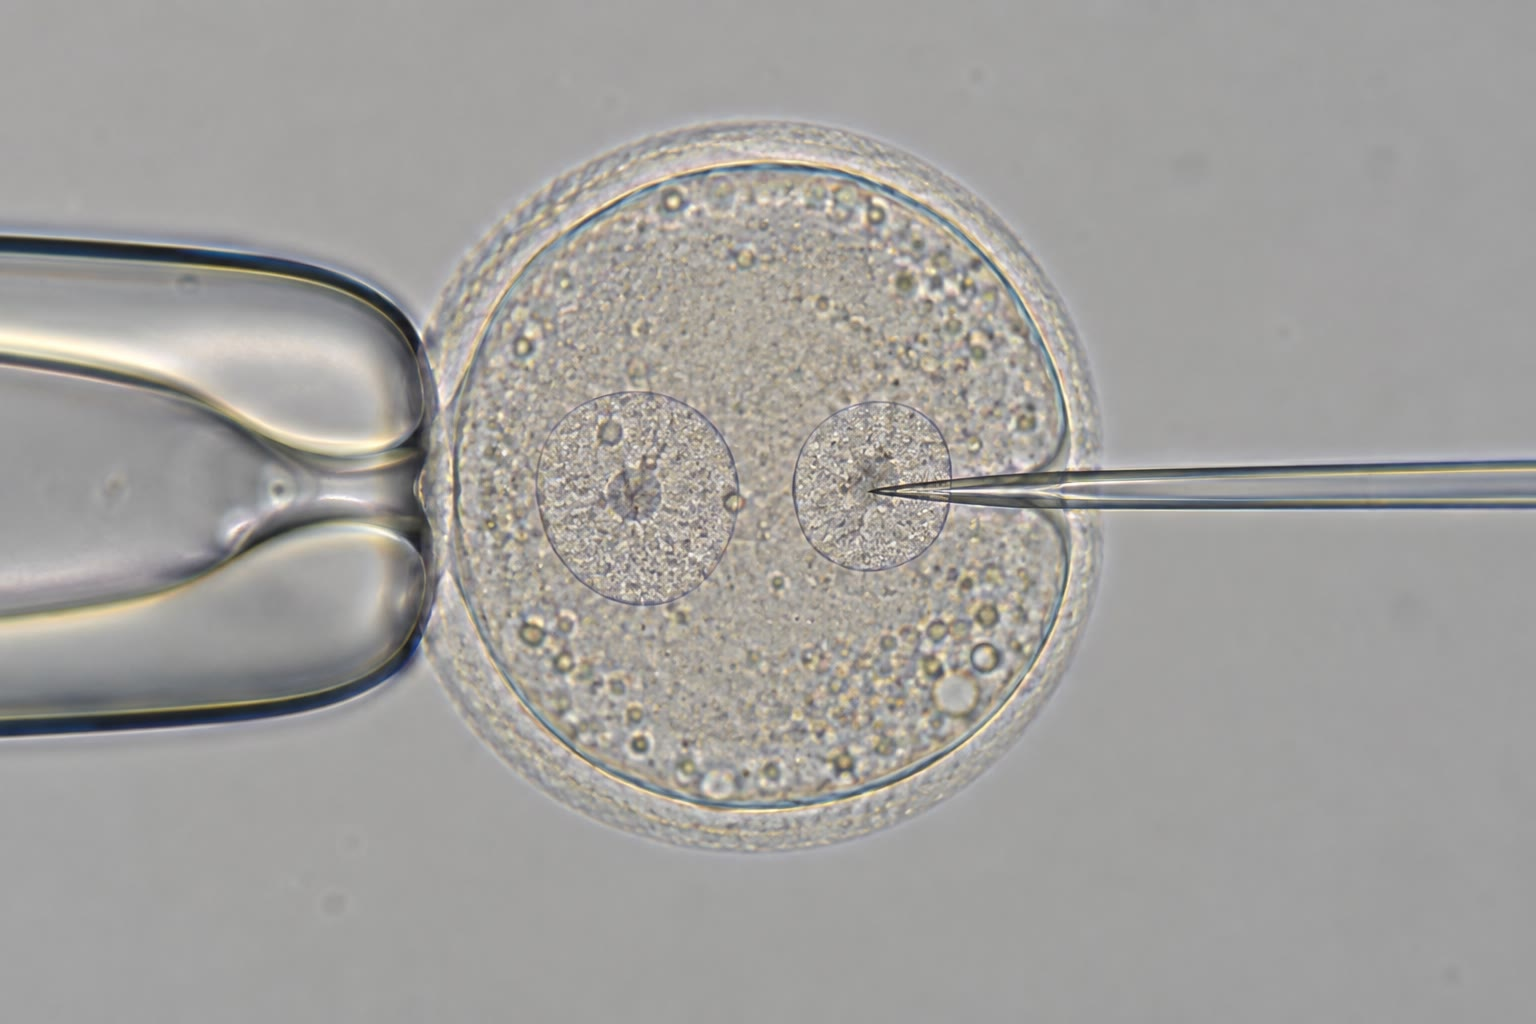
\includegraphics[width=0.46\linewidth]{images/book5/ai/b5-06-microinjection.jpg}\hspace{0.04\linewidth}
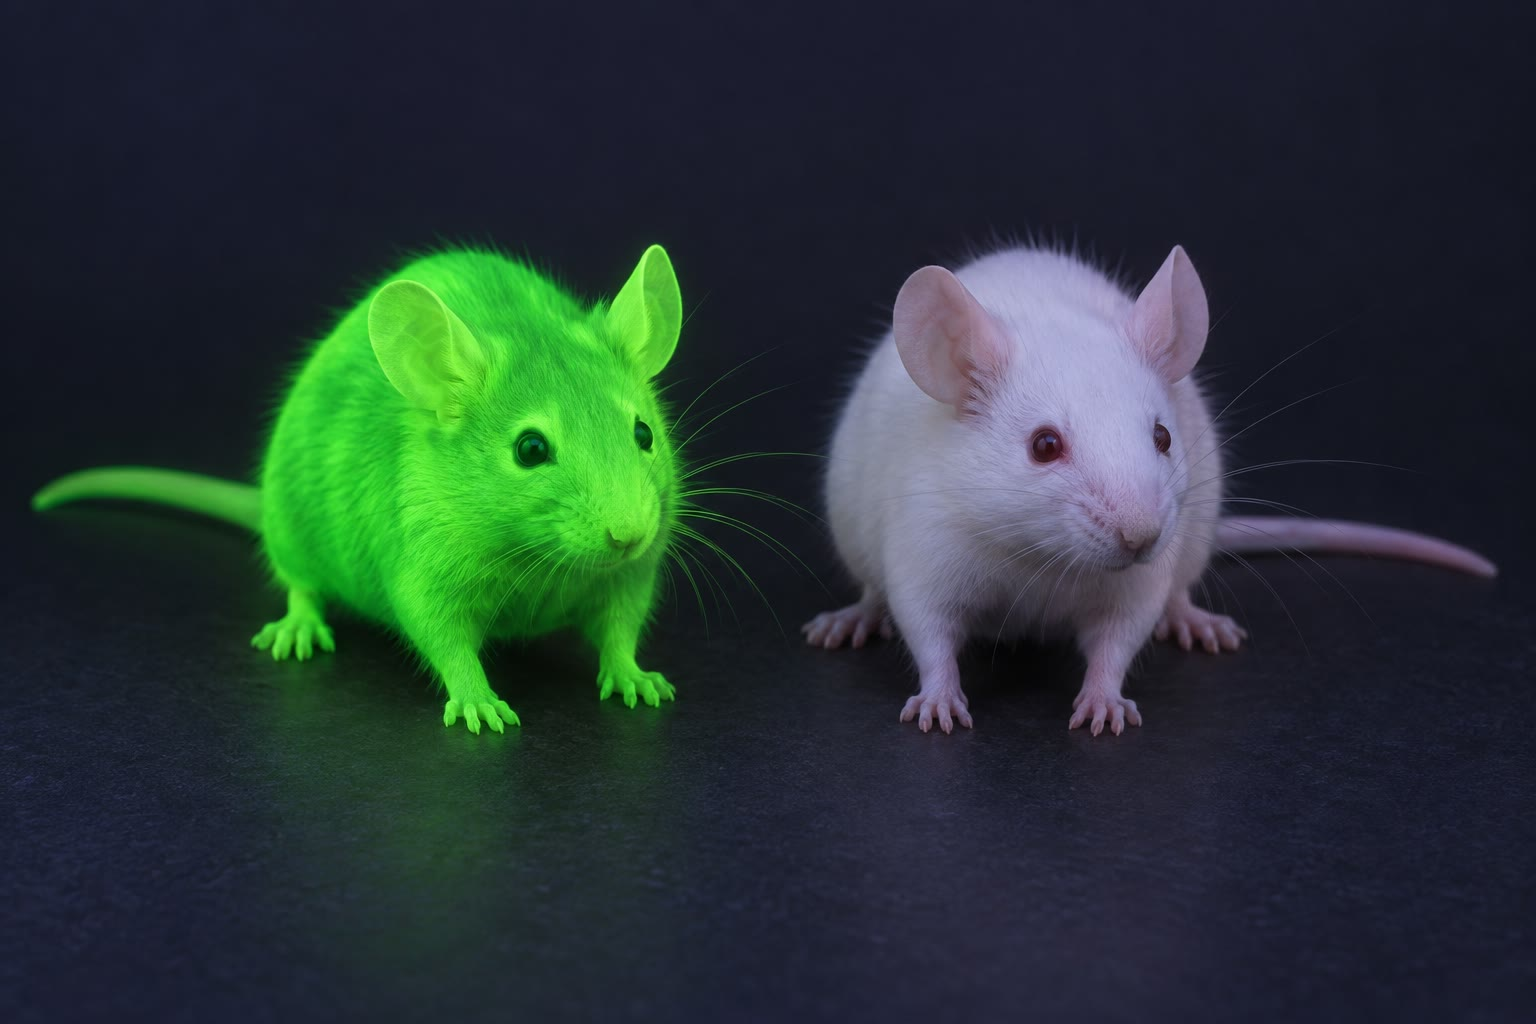
\includegraphics[width=0.46\linewidth]{images/book5/ai/b5-06-gfp-mouse.jpg}

{\small Izquierda: un huevo de ratón fecundado sujeto por succión
mientras una aguja de vidrio inyecta ADN en uno de los pronúcleos.
Derecha: un ratón \omterm{def:b3:genetic-engineering:transgenic}{transgénico} que expresa en todas sus células la
proteína verde fluorescente de una medusa, junto a un hermano de camada
corriente, bajo luz ultravioleta.}
\end{omfigure}

\begin{definition}[Plantas transgénicas]\label{def:b3:genetic-engineering:plants}
\index{Agrobacterium}\index{ADN-T}\index{cultivo modificado genéticamente}
Las plantas se transforman con \emph{Agrobacterium tumefaciens}, una
bacteria del suelo que inserta de forma natural un segmento de su
\omterm{def:b3:genetic-engineering:tools}{plásmido} inductor de tumores, el \emph{ADN-T}, en el genoma de una planta
herida para que forme una agalla y alimente a la bacteria. Sustituir los
genes propios del ADN-T por cualquier gen elegido, entre las secuencias
de borde que la bacteria reconoce, convierte al patógeno en un \omterm{def:b3:genetic-engineering:tools}{vector};
las células transformadas se seleccionan y se regeneran en plantas
enteras, cosa que toda célula vegetal puede hacer. Las especies a las que
la bacteria no infecta (los cereales, durante mucho tiempo) se
transforman disparando partículas de oro recubiertas de ADN contra el
tejido. Los \emph{cultivos modificados genéticamente} que se siembran a
gran escala llevan un gen de toxina bacteriana (\emph{Bt}) contra las
larvas de insecto, o una enzima bacteriana que confiere tolerancia a un
herbicida, o ambos; el \emph{arroz dorado} lleva dos genes de la ruta de
los carotenoides (una fitoeno-sintasa vegetal y una desaturasa
bacteriana) para que su endospermo fabrique $\beta$-caroteno, el
precursor de la vitamina~A, cuya carencia ciega y mata a varios
centenares de miles de niños al año.
\end{definition}

\begin{omfigure}
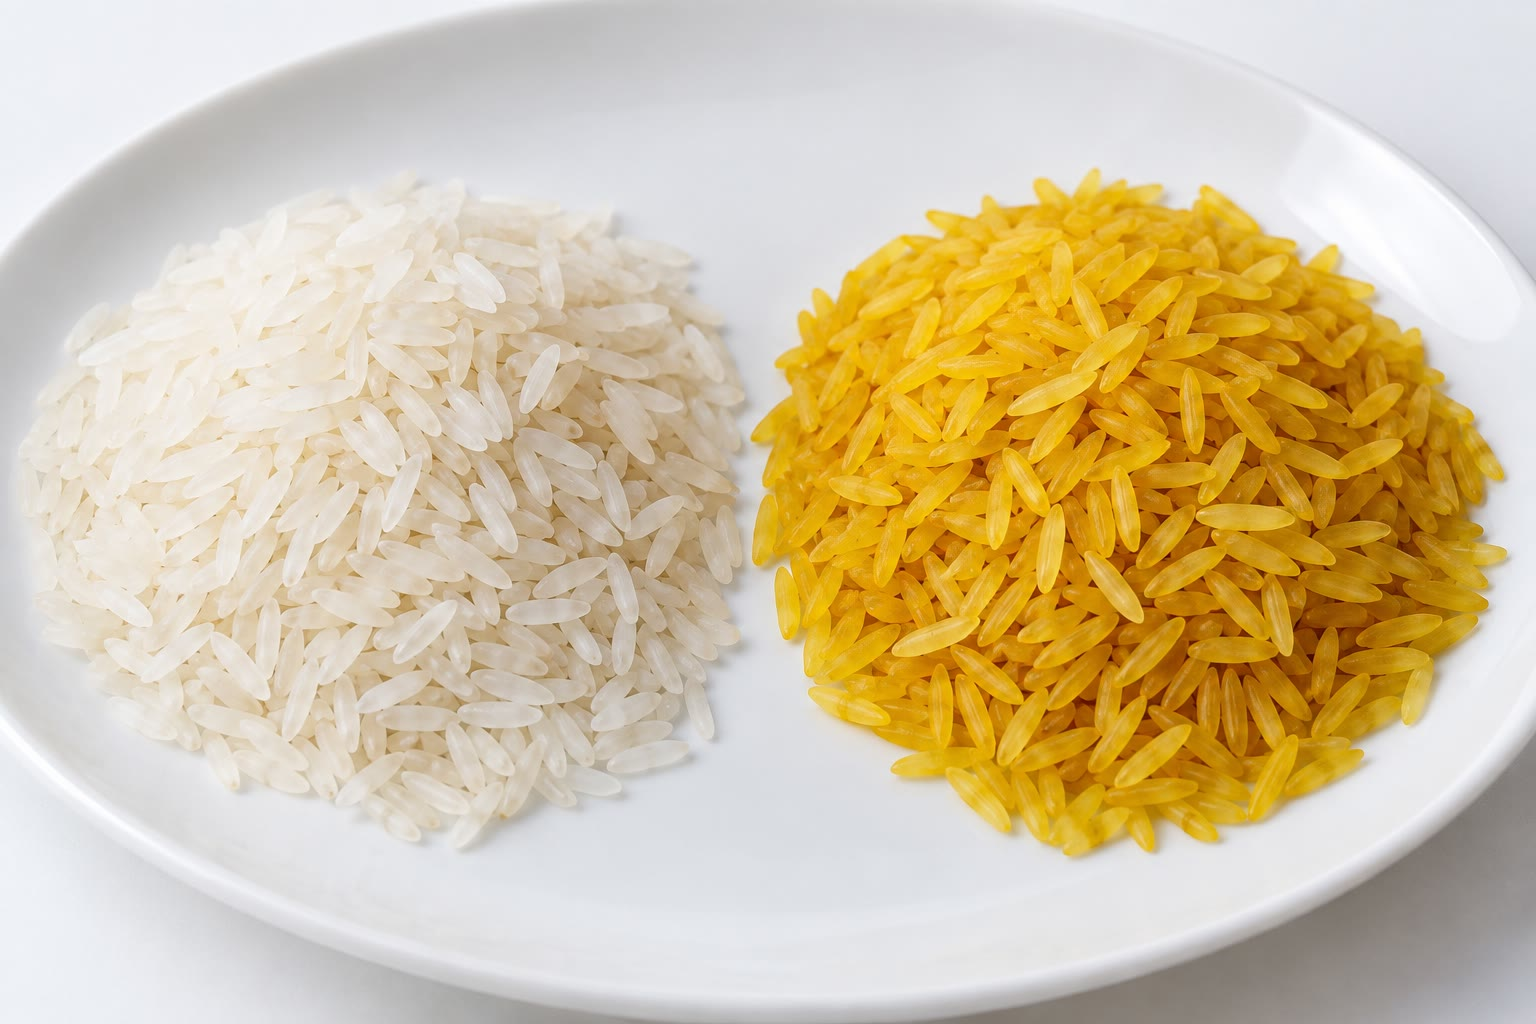
\includegraphics[width=0.46\linewidth]{images/book5/ai/b5-06-golden-rice.jpg}\hspace{0.04\linewidth}
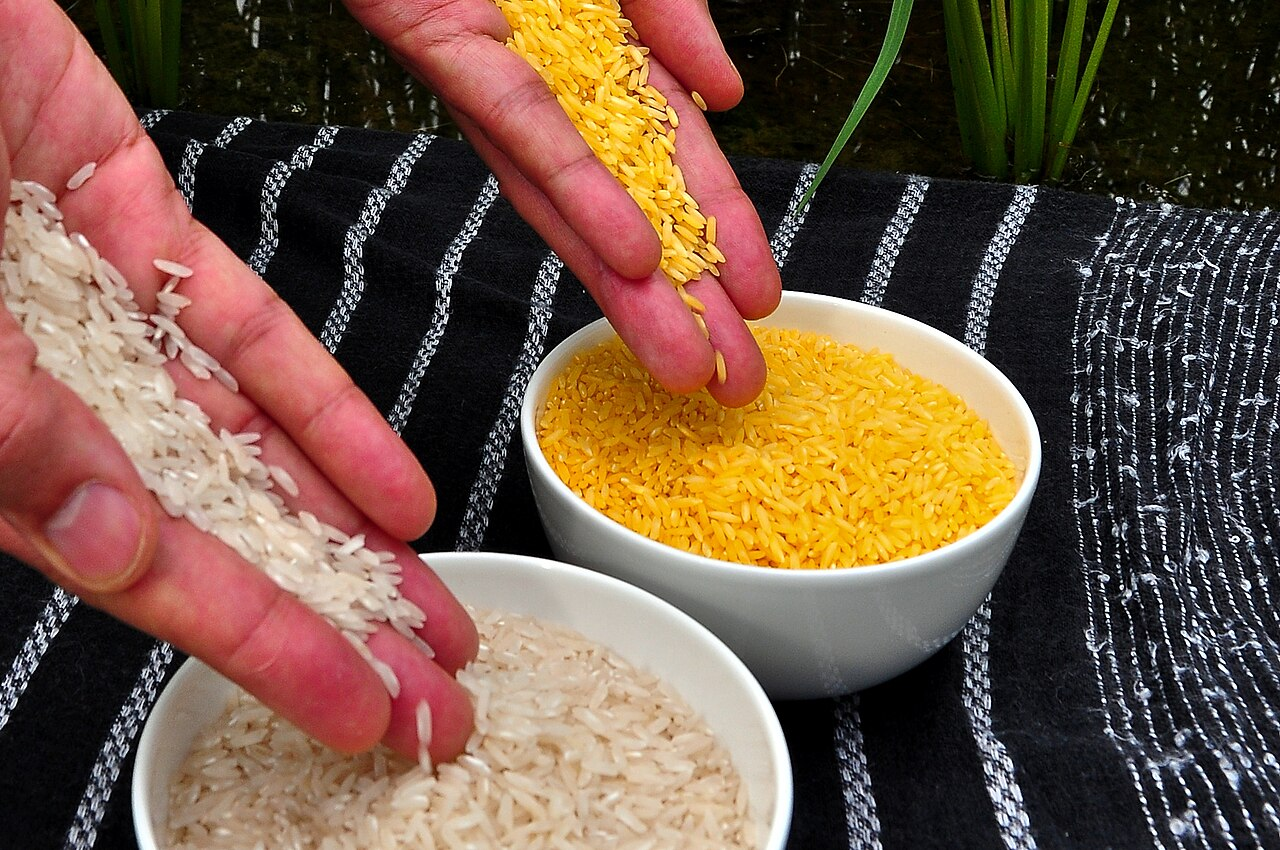
\includegraphics[width=0.46\linewidth]{images/book5/golden-rice-irri.jpg}

{\small Arroz corriente y arroz dorado. El grano amarillo fabrica
$\beta$-caroteno en su endospermo a partir de dos genes añadidos de la
ruta de los carotenoides. Derecha: los dos arroces comparados en el
Instituto Internacional de Investigación del Arroz (IRRI, CC~BY~2.0).}
\end{omfigure}

\begin{remark}[El debate]\label{rem:b3:genetic-engineering:gmo}
Treinta años de cultivo en centenares de millones de hectáreas, y todas
las revisiones sistemáticas de las academias científicas, no han hallado
ningún efecto sobre la salud de los cultivos \omterm{def:b3:genetic-engineering:transgenic}{transgénicos} aprobados que
difiera del de sus equivalentes convencionales; el transgén es un gen más
entre cuarenta mil, y la proteína que fabrica se somete a las mismas
pruebas que cualquier aditivo alimentario. Las cuestiones de verdad son
ecológicas y económicas: la propagación de la resistencia en plagas y
malas hierbas bajo una selección uniforme, el flujo de genes hacia
parientes silvestres, la concentración del mercado de semillas y quién
sale ganando. Son las cuestiones que plantea cualquier tecnología
agrícola potente, y las respuestas dependen del carácter y del contexto,
no del método con el que se movió el gen.
\end{remark}

\section{Editar genomas}

\begin{definition}[CRISPR--Cas9]\label{def:b3:genetic-engineering:crispr}
\index{CRISPR}\index{Cas9}\index{ARN guía}\index{PAM}\index{edición del genoma}
Las bacterias guardan fragmentos de los genomas de los fagos que
infectaron a sus antepasados en una serie de repeticiones (\emph{CRISPR}),
los transcriben en ARN guía cortos y los usan para dirigir una nucleasa
que corte todo ADN correspondiente que entre en la célula: un sistema
inmunitario adaptativo con memoria genética. En \emph{Streptococcus
pyogenes} la nucleasa es una sola proteína, \emph{Cas9}, que se une a un
ARN guía y a un segundo ARN pequeño, rastrea el ADN en busca de un
\emph{\omterm{def:b3:bioinformatics:motif}{motivo} adyacente al protoespaciador} de tres bases (PAM,
5$'$-NGG), desenrolla el ADN contiguo y, si las veinte bases vecinas al
PAM se aparean con la guía, corta las dos hebras a tres bases del PAM.
Jinek, Charpentier, Doudna y colaboradores (2012) fusionaron los dos ARN
en un solo \emph{ARN guía único} y mostraron que Cas9 con una guía de
cualquier secuencia elegida corta el ADN en esa secuencia en un tubo de
ensayo; en menos de un año se había demostrado que la pareja funciona en
células humanas, de ratón, de pez cebra, de planta y de levadura. La
\emph{edición del genoma} es lo que la célula hace con el corte: la unión
de extremos deja una inserción o deleción pequeña que estropea el gen
(una \omterm{def:b3:genetic-engineering:transgenic}{supresión génica} en un paso, en cualquier organismo, en semanas), y
la \omterm{def:b3:dna-repair:dsb}{recombinación homóloga} con un molde aportado escribe una secuencia
elegida.
\end{definition}

\begin{omfigure}
\begin{tikzpicture}[every node/.style={font=\scriptsize}, >=stealth]
  % Cas9 outline (drawn first so labels stay on top)
  \draw[thick, omExo, fill=omExo!15] (5.9,1.1) ellipse (2.6 and 1.6);
  \node[omExo!60!black] at (7.7,2.3) {Cas9};
  % target DNA
  \draw[very thick, omDef] (0,0.3) -- (11,0.3); \draw[very thick, omDef] (0,-0.1) -- (11,-0.1);
  % PAM
  \fill[omProp!60] (7.2,-0.2) rectangle (7.9,0.4); \node[below] at (7.55,-0.25) {PAM (NGG)};
  % protospacer
  \draw[omThm, very thick] (4.2,0.5) -- (7.15,0.5); \node[above] at (5.7,0.55) {diana de 20 bases, apareada con la guía};
  % guide RNA
  \draw[very thick, omMeth!70!black] (4.2,0.3) .. controls (4.2,1.6) and (5.0,1.9) .. (5.4,1.9) -- (6.6,1.9) .. controls (7.0,1.9) and (7.2,2.5) .. (6.8,2.8) .. controls (6.3,3.1) and (5.8,2.7) .. (6.1,2.4);
  \node[left, omMeth!70!black, align=right] at (3.2,2.2) {ARN guía único:\\20 bases a elección\\+ horquilla de unión a Cas9};
  % cut
  \draw[omThm, very thick, ->] (6.25,-0.7) -- (6.25,0.35); \node[omThm, below] at (6.25,-0.7) {rotura de doble hebra, a 3 bases del PAM};
  % outcomes
  \draw[->, thick] (2.0,-1.3) -- (2.0,-1.9); \node[below, align=center] at (2.0,-1.9) {unión de extremos:\\inserción o deleción pequeña\\$\Rightarrow$ cambio de marco, supresión};
  \draw[->, thick] (10.0,-1.3) -- (10.0,-1.9); \node[below, align=center] at (10.0,-1.9) {recombinación con un\\molde aportado\\$\Rightarrow$ cambio preciso};
\end{tikzpicture}

{\small \omterm{def:b3:genetic-engineering:crispr}{Cas9} y su guía. La proteína se une a un \omterm{def:b3:genetic-engineering:crispr}{PAM}, desenrolla el ADN
contiguo y corta si las veinte bases se aparean con el \omterm{def:b3:genetic-engineering:crispr}{ARN guía}. La
rotura se repara o bien por unión de extremos, que estropea el gen, o
bien por recombinación con un molde, que lo reescribe.}
\end{omfigure}

\begin{proposition}[Editar sin rotura]\label{prop:b3:genetic-engineering:editors}
\index{editor de bases}\index{editor cebado}\index{fuera de diana}
Cortar las dos hebras es la edición más tosca: el resultado de la unión
de extremos es aleatorio, y una rotura en otro sitio --- un lugar
\emph{\omterm{prop:b3:genetic-engineering:editors}{fuera de diana}} que difiere de la guía en unas pocas posiciones y
que \omterm{def:b3:genetic-engineering:crispr}{Cas9} tolera --- es una mutación que nadie ha pedido. Una \omterm{def:b3:genetic-engineering:crispr}{Cas9} con un
dominio nucleasa inactivado muerde una sola hebra; con los dos
inactivados se limita a unirse, y puede llevar otras enzimas hasta una
secuencia. Los \emph{\omterm{prop:b3:genetic-engineering:editors}{editores de bases}} fusionan una \omterm{def:b3:genetic-engineering:crispr}{Cas9} mordedora con
una desaminasa que convierte C en U (leída como T) o A en I (leída como
G) en la hebra desenrollada, y cambian una base sin rotura y sin molde;
los \emph{\omterm{prop:b3:genetic-engineering:editors}{editores cebados}} llevan una transcriptasa inversa y una guía
alargada con la secuencia deseada, y copian esa secuencia en la hebra
mordida, lo que permite cualquier sustitución y pequeñas inserciones o
deleciones. La actividad \omterm{prop:b3:genetic-engineering:editors}{fuera de diana} se reduce con variantes de \omterm{def:b3:genetic-engineering:crispr}{Cas9}
de alta fidelidad diseñadas a tal efecto, entregando la enzima brevemente
como proteína en lugar de como gen, y eligiendo guías cuyos parientes
genómicos más próximos difieran en varias posiciones; se mide
secuenciando los sitios predichos y con métodos sin sesgo que captan toda
rotura del genoma.
\end{proposition}

\begin{example}[Una cura]\label{ex:b3:genetic-engineering:sickle}
La anemia falciforme es un cambio de una sola base en la
$\beta$-globina. La hemoglobina fetal, hecha de $\gamma$-globina,
serviría de sustituta, pero los genes $\gamma$ los apaga tras el
nacimiento el represor BCL11A. La primera terapia \omterm{def:b3:genetic-engineering:crispr}{CRISPR} aprobada (2023)
toma las propias células madre sanguíneas del paciente, corta con \omterm{def:b3:genetic-engineering:crispr}{Cas9} el
potenciador eritroide de \emph{BCL11A} de modo que la unión de extremos
lo inutilice en la mayoría de las células, y devuelve las células después
de vaciar la médula del paciente: los glóbulos rojos que fabrican son
ricos en hemoglobina fetal, no se falciforman y las crisis cesan. La
edición es somática --- la línea germinal queda intacta y el cambio no se
hereda --- y usa el resultado ``tosco'', la interrupción, allí donde lo
que se quiere es interrumpir.
\end{example}

\begin{theorem}[Propagación supramendeliana de un impulsor génico]\label{thm:b3:genetic-engineering:drive}
\index{impulsor génico}
Un \emph{\omterm{thm:b3:genetic-engineering:drive}{impulsor génico}} es una construcción que codifica una \omterm{def:b3:genetic-engineering:crispr}{Cas9} y una
guía que corta el alelo silvestre en su propio locus en un heterocigoto;
la reparación por recombinación copia el impulsor en el cromosoma
cortado, de modo que una fracción $c$ de los gametos del heterocigoto
lleva el impulsor en lugar de la mitad mendeliana. Si el impulsor tiene
frecuencia $p$ en una población grande con apareamiento al azar y no
tiene coste de eficacia biológica, su frecuencia en la generación
siguiente es
\[
p' = p + c\,p\,(1 - p),
\]
de modo que se propaga desde la rareza a un ritmo proporcional a $c$ y
alcanza la mitad de la población en unas $\ln(1/p_{0})/\ln(1 + c)$
generaciones desde una frecuencia inicial $p_{0}$.
\end{theorem}
\begin{proof}
El apareamiento al azar da homocigotos del impulsor con frecuencia
$p^{2}$, heterocigotos con $2p(1-p)$ y homocigotos silvestres con
$(1-p)^{2}$. Los homocigotos transmiten el impulsor a todos sus gametos,
los heterocigotos a una fracción $(1 + c)/2$ (la mitad por Mendel, más
$c$ veces la mitad silvestre convertida) y los silvestres a ninguno. De
ahí que $p' = p^{2} + 2p(1-p)(1+c)/2
= p^{2} + p(1-p) + c\,p(1-p) = p + c\,p(1-p)$. Para $p$ pequeño esto es
$p' \approx (1+c)p$, un crecimiento geométrico de razón $1 + c$, que
alcanza $1/2$ desde $p_{0}$ tras unas $\ln(1/2p_{0})/\ln(1+c)$
generaciones; el término logístico solo lo frena cerca del final.
\end{proof}

\begin{omfigure}
\begin{tikzpicture}
\begin{axis}[
  width=0.7\linewidth, height=5.6cm,
  axis x line=bottom, axis y line=left,
  xmin=0, xmax=20, ymin=0, ymax=1.05,
  xlabel={generación}, ylabel={frecuencia del impulsor $p$},
  xlabel style={font=\small, at={(axis description cs:0.5,-0.12)}, anchor=north},
  ylabel style={font=\small},
  tick label style={font=\small}, xtick={0,5,10,15,20}, ytick={0,0.5,1},
  clip=false,
]
\addplot[very thick, omThm, mark=*, mark size=1.2pt] coordinates {(0,0.01) (1,0.0189) (2,0.0356) (3,0.0665) (4,0.1224) (5,0.2191) (6,0.3731) (7,0.5836) (8,0.8023) (9,0.9451) (10,0.9918) (11,0.9991) (12,1.0) (13,1.0) (14,1.0) (15,1.0) (16,1.0) (17,1.0) (18,1.0) (19,1.0) (20,1.0)};
\addplot[very thick, omDef, mark=*, mark size=1.2pt] coordinates {(0,0.01) (1,0.015) (2,0.0223) (3,0.0332) (4,0.0493) (5,0.0727) (6,0.1064) (7,0.154) (8,0.2191) (9,0.3047) (10,0.4106) (11,0.5316) (12,0.6561) (13,0.769) (14,0.8578) (15,0.9188) (16,0.9561) (17,0.9771) (18,0.9883) (19,0.9941) (20,0.997)};
\addplot[very thick, gray, dashed, domain=0:20, samples=2] {0.01};
\node[font=\scriptsize, omThm, anchor=south east] at (axis cs:6.5,0.62) {$c = 0.9$};
\node[font=\scriptsize, omDef, anchor=north west] at (axis cs:12.5,0.62) {$c = 0.5$};
\node[font=\scriptsize, gray, anchor=south west] at (axis cs:12,0.02) {mendeliano, $c = 0$: se queda en $p_{0}$};
\end{axis}
\end{tikzpicture}

{\small Un \omterm{thm:b3:genetic-engineering:drive}{impulsor génico} liberado al uno por ciento, con eficiencia de
conversión $0.9$ o $0.5$ y sin coste de eficacia biológica. Un alelo
mendeliano sin ventaja se quedaría en el uno por ciento; el impulsor se
adueña de la población en diez o veinte generaciones.}
\end{omfigure}

\begin{remark}[Qué puede editarse]\label{rem:b3:genetic-engineering:ethics}
Editar las células somáticas de un paciente que da su consentimiento es
medicina, y se juzga como cualquier tratamiento por sus riesgos y sus
beneficios. Editar la línea germinal --- un embrión, cuya descendencia
entera llevaría el cambio --- es distinto en su naturaleza: la persona
afectada no puede consentir, el cambio se hereda y los resultados \omterm{prop:b3:genetic-engineering:editors}{fuera
de diana} y en mosaico de la técnica aún no están controlados; después de
que un científico chino anunciara en 2018 que lo había hecho en unas
gemelas, las academias científicas de la mayoría de los países pidieron
una moratoria y varios Estados lo tipificaron como delito. Un \omterm{thm:b3:genetic-engineering:drive}{impulsor
génico} liberado en una población silvestre es una decisión tomada en
nombre de todos los que vengan después, y por eso las propias propuestas
del campo para eliminar los mosquitos del paludismo acompañan los
impulsores de salvaguardas --- impulsores de reversión, diseños
autolimitados --- y del consentimiento público de los países afectados.
\end{remark}

\section{Ejercicios}

\begin{exercise}[$\star$]\label{exo:b3:genetic-engineering:1}
Enumérense los tres componentes que debe tener un \omterm{def:b3:genetic-engineering:tools}{plásmido} de clonación y
explíquese la finalidad de cada uno.
\end{exercise}

\begin{exercise}[$\star$]\label{exo:b3:genetic-engineering:2}
EcoRI reconoce GAATTC. ¿Con qué frecuencia aparece el sitio, en promedio,
en ADN aleatorio, y cuántos fragmentos produce del genoma de
\emph{E.~coli} de \qty{4.6}{Mb}? ¿Por qué el número real es algo distinto?
\end{exercise}

\begin{exercise}[$\star$]\label{exo:b3:genetic-engineering:3}
Enúnciense los tres pasos de temperatura de un ciclo de PCR y qué ocurre
en cada uno. ¿Por qué ha de ser termoestable la polimerasa?
\end{exercise}

\begin{exercise}[$\star$]\label{exo:b3:genetic-engineering:4}
¿Qué necesita \omterm{def:b3:genetic-engineering:crispr}{Cas9} para cortar una secuencia dada, y qué dos resultados
pueden seguir al corte?
\end{exercise}

\begin{exercise}[$\star\star$]\label{exo:b3:genetic-engineering:5}
Una PCR corre $35$ ciclos con eficiencia $E = 0.9$ a partir de $50$
copias. ¿Cuántas copias resultan? Una qPCR de dos muestras da
$C_{T} = 18.2$ y $25.5$; con $E = 0.95$, ¿cuál es la razón de sus
cantidades iniciales?
\end{exercise}

\begin{exercise}[$\star\star$]\label{exo:b3:genetic-engineering:6}
¿Por qué se usa una genoteca de ADNc, y no una genómica, para expresar
una proteína humana en bacterias? Nómbrense otros dos obstáculos para
fabricar una proteína humana en \emph{E.~coli} y dígase cómo se salva
cada uno.
\end{exercise}

\begin{exercise}[$\star\star$]\label{exo:b3:genetic-engineering:7}
Se fabrica un ratón con \omterm{def:b3:genetic-engineering:transgenic}{supresión génica} por direccionamiento en \omterm{def:b3:genetic-engineering:transgenic}{células
madre embrionarias}. Explíquese por qué el primer ratón que nace es una
quimera, por qué hay que cruzarlo y qué fracción de los nietos de una
quimera cuya línea germinal está dirigida a medias son homocigotos para
la supresión si se intercruzan abuelos heterocigóticos.
\end{exercise}

\begin{exercise}[$\star\star$]\label{exo:b3:genetic-engineering:8}
Se elige un \omterm{def:b3:genetic-engineering:crispr}{ARN guía} de 20 bases con un \omterm{def:b3:genetic-engineering:crispr}{PAM} NGG. ¿Cuántos sitios de un
genoma de $3.2\times 10^{9}$ bp (ambas hebras) coinciden por azar
exactamente con la guía? ¿Cuántos coinciden con hasta dos discrepancias,
si \omterm{def:b3:genetic-engineering:crispr}{Cas9} las tolera? (Cuéntense las secuencias a dos discrepancias como
$1 + 3\binom{20}{1} +
9\binom{20}{2}$.)
\end{exercise}

\begin{exercise}[$\star\star$]\label{exo:b3:genetic-engineering:9}
Con el \cref{thm:b3:genetic-engineering:drive}, calcúlese la frecuencia
de un impulsor con $c = 0.8$ tras tres generaciones desde $p_{0} = 0.05$,
y estímese el número de generaciones para llegar a $0.5$.
\end{exercise}

\begin{exercise}[$\star\star\star$]\label{exo:b3:genetic-engineering:10}
La terapia de la anemia falciforme interrumpe un potenciador en lugar de
corregir la mutación de la $\beta$-globina. Dense dos razones por las que
se eligió la interrupción por unión de extremos frente a la corrección
por \omterm{def:b3:dna-repair:dsb}{recombinación homóloga} en células madre sanguíneas, y un
inconveniente.
\end{exercise}

\begin{exercise}[$\star\star\star$]\label{exo:b3:genetic-engineering:11}
Un \omterm{thm:b3:genetic-engineering:drive}{impulsor génico} contra un mosquito lleva un coste de eficacia
biológica $s$ en los homocigotos. Modifíquese la recurrencia para
incluir la selección contra los homocigotos del impulsor y hállese la
condición sobre $c$ y $s$ para que el impulsor se propague desde la
rareza. Explíquese después por qué los alelos de resistencia ---
productos de la unión de extremos en la diana que la guía ya no reconoce
--- son el principal obstáculo en la práctica.
\end{exercise}

\begin{exercise}[$\star\star\star$]\label{exo:b3:genetic-engineering:12}
Arguméntese, con los mecanismos de este capítulo y del
\cref{ch:b3:dna-repair}, por qué la edición de la línea germinal de un
embrión humano no puede garantizar hoy el resultado pretendido en todas
las células, y qué pruebas harían falta antes de que una persona racional
pudiera considerarla segura.
\end{exercise}

\section{Problema: de un gen a un fármaco y a un cultivo}

\begin{problem}[{Problema de fin de semana --- un gen clonado con la
aritmética de los sitios de restricción y de la transformación, un virus
contado por qPCR, una hormona producida por toneladas en un fermentador,
un genoma editado con sus dianas erróneas contadas y un impulsor génico
cronometrado, hasta llegar a las copias de un virus en una muestra, al
volumen anual de fermentador para la insulina del mundo y al número de
generaciones que necesita un impulsor}]
\label{pb:b3:genetic-engineering:1}
Datos: un gen de \qty{1.5}{kb}; un sitio de restricción de seis bases; un
\omterm{def:b3:genetic-engineering:tools}{plásmido} de \qty{4}{kb}; eficiencia de transformación, $2\times 10^{7}$
colonias por microgramo de \omterm{def:b3:genetic-engineering:tools}{plásmido}; la ligación da inserto al
\qty{10}{\%} de los \omterm{def:b3:genetic-engineering:tools}{plásmidos}. Eficiencia de la qPCR $E = 1$, umbral
$N_{T} = 10^{12}$. Insulina: \qty{5.8}{kDa}; un paciente usa $40$
unidades al día, y una unidad son \qty{35}{\micro g}; $10^{7}$ pacientes;
un fermentador rinde \qty{2}{g/L} de producto por tanda, con diez tandas
al año. Genoma, $3.2\times
10^{9}$ bp. Conversión del impulsor $c = 0.9$, liberado a $p_{0} = 0.001$.

\medskip
\noindent\textbf{Parte I --- Clonación.}
\begin{enumerate}
  \item ¿Con qué frecuencia aparece un sitio dado de seis bases en ADN
        aleatorio? ¿Cuál es la probabilidad de que el gen de
        \qty{1.5}{kb} no contenga ningún sitio de esos, de modo que la
        enzima pueda usarse para clonarlo entero?
  \item Si sí contiene un sitio, ¿cómo se clonaría de todos modos? (Dos
        métodos.)
  \item Se transforman \qty{100}{ng} de \omterm{def:b3:genetic-engineering:tools}{plásmido} ligado. ¿Cuántas
        colonias, y cuántas llevan el inserto?
  \item Se usa el cribado azul--blanco. ¿Qué fracción de las colonias es
        blanca, y cuántas colonias blancas hay que tomar para tener un
        \qty{99}{\%} de probabilidad de que al menos una lleve el gen en
        la orientación correcta (la mitad de los insertos)?
  \item El \omterm{def:b3:genetic-engineering:tools}{plásmido} recombinante mide \qty{5.5}{kb}. Una célula contiene
        $50$ copias y se divide cada \qty{30}{min}. Tras un crecimiento
        nocturno (\qty{16}{h}) desde una sola célula, ¿cuántas moléculas
        de \omterm{def:b3:genetic-engineering:tools}{plásmido}, y qué masa de ADN plasmídico (\qty{650}{Da} por par
        de bases)?
  \item ¿Por qué el \omterm{def:b3:genetic-engineering:tools}{plásmido} necesita un origen bacteriano mientras que
        el gen humano insertado no necesita promotor bacteriano para
        clonarse, pero sí para expresarse?
\end{enumerate}

\medskip
\noindent\textbf{Parte II --- Contar un virus.}
\begin{enumerate}[resume]
  \item La muestra de un paciente cruza el umbral en $C_{T} = 28$.
        ¿Cuántas copias había en la reacción? ¿Y en otra con
        $C_{T} = 35$?
  \item Sensibilidad: ¿cuántos ciclos hacen falta para llevar una sola
        copia hasta el umbral?
  \item El punto de corte de la prueba se fija en $C_{T} = 38$. ¿A qué
        número de copias corresponde, y por qué no usar $45$ ciclos?
  \item Una molécula contaminante del producto de una carrera anterior
        entra en una muestra negativa. ¿En qué ciclo cruza el umbral?
        ¿Qué práctica de laboratorio lo evita?
  \item La transcripción inversa convierte en ADN el \qty{40}{\%} del
        ARN vírico. Corríjase el recuento de la pregunta 7 para la
        primera muestra.
  \item Dos muestras difieren en $\Delta C_{T} = 3.3$ con $E = 1$, pero
        la eficiencia es en realidad $0.9$. ¿Qué diferencia de veces
        informa el analista, y cuál es la verdadera?
\end{enumerate}

\medskip
\noindent\textbf{Parte III --- Insulina por toneladas.}
\begin{enumerate}[resume]
  \item Calcúlense la masa diaria de insulina por paciente y la
        necesidad mundial anual para $10^{7}$ pacientes, en kilogramos.
  \item ¿Cuántos moles de insulina son, y cuántas moléculas?
  \item ¿Qué volumen de fermentador, con diez tandas al año, la produce?
        Compárese con una piscina de \qty{2500}{m^3}.
  \item La extracción de glándulas daba \qty{1}{kg} de insulina por cada
        \qty{8000}{kg} de páncreas; un páncreas de cerdo pesa
        \qty{100}{g}. ¿Cuántos cerdos al año necesitaría el mundo?
  \item ¿Por qué se prefiere la hormona recombinante incluso donde la
        insulina animal es barata? Dense dos razones.
  \item Los análogos de la insulina difieren de la secuencia humana en
        uno o dos residuos. Explíquese por qué un análogo sigue siendo
        un fármaco que actúa sobre el receptor humano, y por qué el
        cambio de un solo residuo puede alterar su tiempo de
        disociación.
\end{enumerate}

\medskip
\noindent\textbf{Parte IV --- Editar e impulsar.}
\begin{enumerate}[resume]
  \item ¿Cuántas coincidencias exactas de una guía de 20 bases más NGG
        contiene el genoma por azar (ambas hebras: $6.4\times 10^{9}$
        posiciones)?
  \item Si \omterm{def:b3:genetic-engineering:crispr}{Cas9} tolera hasta tres discrepancias, ¿cuántas secuencias
        están a tres discrepancias de la guía, y cuántos sitios \omterm{prop:b3:genetic-engineering:editors}{fuera de
        diana} por azar resultan?
  \item Las células madre sanguíneas editadas son $10^{7}$; el
        \qty{80}{\%} lleva la interrupción pretendida. ¿Cuántas células
        llevan una rotura \omterm{prop:b3:genetic-engineering:editors}{fuera de diana} en un sitio dado si se corta en
        una célula de cada $10^{4}$, y por qué preocupa una rotura en un
        gen supresor de tumores en una sola célula madre?
  \item Calcúlese la frecuencia del impulsor tras $1, 2, 3$
        generaciones desde $p_{0} = 0.001$, y estímense las generaciones
        hasta $0.5$.
  \item Un mosquito tiene diez generaciones al año. ¿Cuántos años tarda
        en adueñarse de la población? ¿Cómo cambia cualitativamente el
        panorama un coste de eficacia biológica del \qty{20}{\%} en los
        homocigotos?
  \item Un alelo de resistencia surge cuando el corte lo repara la unión
        de extremos y no la recombinación, con probabilidad $1 - c = 0.1$
        por intento de conversión. Estímese el número de alelos de
        resistencia creados en una población de $10^{6}$ heterocigotos en
        una generación, y explíquese qué le ocurre al impulsor si son
        biológicamente eficaces.
  \item Resúmase: las copias de la primera muestra (pregunta~7), el
        volumen anual de fermentador para la insulina del mundo
        (pregunta~15) y las generaciones que tarda el impulsor en llegar
        a la mitad de la población (pregunta~22).
\end{enumerate}
\end{problem}
